
%(BEGIN_QUESTION)
% Copyright 2003, Tony R. Kuphaldt, released under the Creative Commons Attribution License (v 1.0)
% This means you may do almost anything with this work of mine, so long as you give me proper credit

There is a problem somewhere in this relay logic circuit.  Lamp 2 operates exactly as it should, but lamp 1 never turns on.  Identify all possible failures in the circuit that could cause this problem, and then explain how you would troubleshoot the problem as efficiently as possible (taking the least amount of electrical measurements to identify the specific problem).

$$\includegraphics[width=15.5cm]{i02320x01.eps}$$

Next, suppose an electrician tried to force lamp 1 to energize by connecting a temporary jumper wire in parallel with that lamp.  Explain why this strategy will {\it not} work, and in fact will likely cause damage to the circuit.

\vskip 20pt \vbox{\hrule \hbox{\strut \vrule{} {\bf Suggestions for Socratic discussion} \vrule} \hrule}

\begin{itemize}
\item{} Identify how ladder-logic type diagrams differ from standard electronic schematics, particularly with regard to how electromechanical relay coils and contacts are shown in each.
\item{} Suppose you were asked to diagnose the problem in this circuit without using any test equipment, but simply by observing and listening to the circuit function.  Knowing that an electromechanical relay typically makes a soft ``click'' sound when its coil changes state, explain how you could isolate certain faults in this circuit without a multimeter.
\item{} Explain why a relay {\it coil} failing shorted will not necessarily yield the same results as a relay {\it contact} failing shorted.
\end{itemize}

\underbar{file i02320}
%(END_QUESTION)





%(BEGIN_ANSWER)

This is a problem worthy of a good in-class discussion with your peers!  Of course, several things could be wrong in this circuit to cause lamp 1 to never energize.  When you explain what measurements you would take in isolating the problem, be sure to describe whether or not you are actuating either of the pushbutton switches when you take those measurements. 

\vskip 10pt

Jumpering across lamp 1 creates a {\it short-circuit} condition by removing the only load in that ``rung'' of the circuit!

%(END_ANSWER)





%(BEGIN_NOTES)

Be sure to leave plenty of classroom time for a discussion on troubleshooting this circuit.  Electrical troubleshooting is a difficult-to-develop skill, and it takes lots of time for some people to acquire.  Being one of the most valuable skills a technical person can possess, it is well worth the time invested!

Some possible problems include:

\begin{itemize}
\item{} Lamp 1 burned out
\item{} Contact CR3-1 failed open
\item{} Broken wire between CR3-1 and Lamp 1
\item{} Contact CR1-1 shorted (assuming contact CR1-2 remains functional)
\item{} Contact CR2-1 shorted (assuming contact CR2-2 remains functional)
\end{itemize}

Two things we know are okay in this circuit are the pushbutton switches, and also relay coils CR1 and CR2.


\vskip 10pt

Jumpering across lamp 1 creates a {\it short-circuit} condition by removing the only load in that ``rung'' of the circuit!  If and when contact CR3-1 closes, the power source will become shorted, either damaging something or blowing the fuse through which power is supplied to this whole circuit.








\vskip 20pt \vbox{\hrule \hbox{\strut \vrule{} {\bf Virtual Troubleshooting} \vrule} \hrule}

This question is a good candidate for a ``Virtual Troubleshooting'' exercise.  Presenting the diagram to students, you first imagine in your own mind a particular fault in the system.  Then, you present one or more symptoms of that fault (something noticeable by an operator or other user of the system).  Students then propose various diagnostic tests to perform on this system to identify the nature and location of the fault, as though they were technicians trying to troubleshoot the problem.  Your job is to tell them what the result(s) would be for each of the proposed diagnostic tests, documenting those results where all the students can see.

During and after the exercise, it is good to ask students follow-up questions such as:

\begin{itemize}
\item{} What does the result of the last diagnostic test tell you about the fault?
\item{} Suppose the results of the last diagnostic test were different.  What then would that result tell you about the fault?
\item{} Is the last diagnostic test the best one we could do?
\item{} What would be the ideal order of tests, to diagnose the problem in as few steps as possible?
\end{itemize}

%INDEX% Relay, diagram: ladder logic

%(END_NOTES)


